\chapter{Design drawings}
In this chapter, the extracts from the design drawings relevant to this Thesis are presented. The general notes on the materials and load combinations are given in Section \ref{app:general_notes}. The cross-sections of the different segments are presented in Section \ref{app:cross_sections}. The weight of the bridge is estimated from the summary of quantities in Section \ref{app:weight}. Ultimately, a summary of the final design verifications is given in Section \ref{app:design_verifications}. The values refer to the American units \SI{}{ft}, \SI{}{in}, \SI{}{kip}, \SI{}{kip ft} and \SI{}{ksi}. The general plan is shown in Fig. \ref{fig:general_plan}.
\begin{figure}[H]
    \centering
    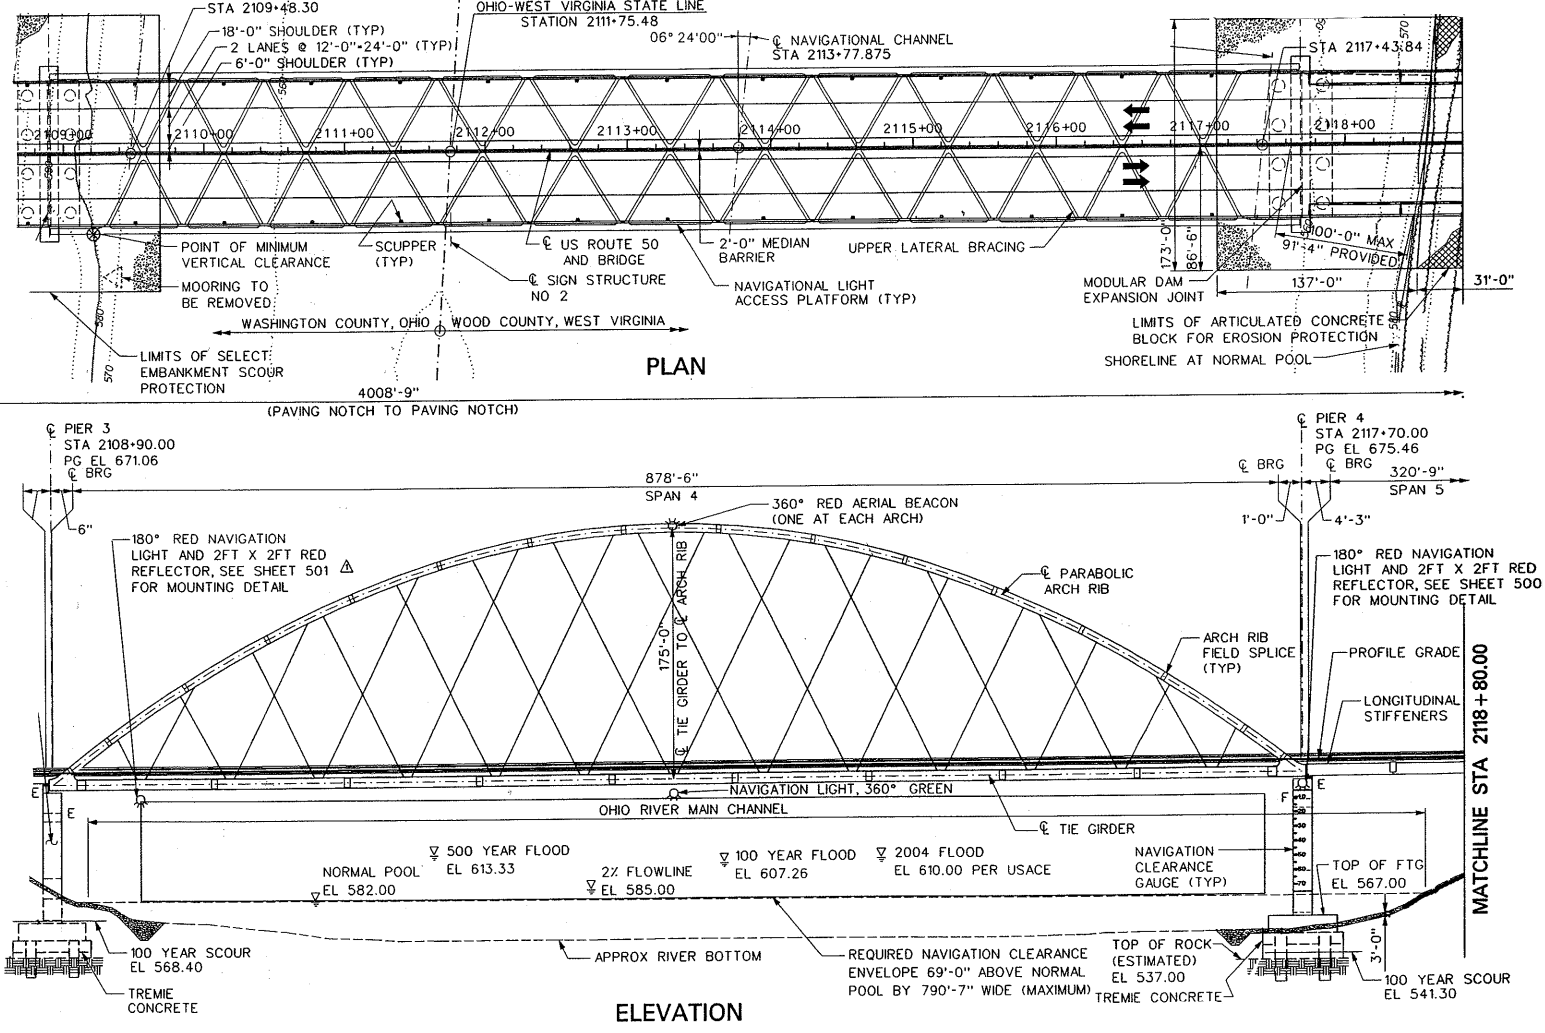
\includegraphics[width=\textwidth]{overleaf/Appendix/Design drawings/General Plan.png}
    \caption{General plan}
    \label{fig:general_plan}
\end{figure}

\newpage
\section{General notes} \label{app:general_notes}
The general notes on the materials, the hanger resistance factors and the load combinations for cable loss and tie fracture are presented in Figs. \ref{fig:materials} to \ref{fig:hanger_load_combination}.
\begin{figure}[H]
    \centering
    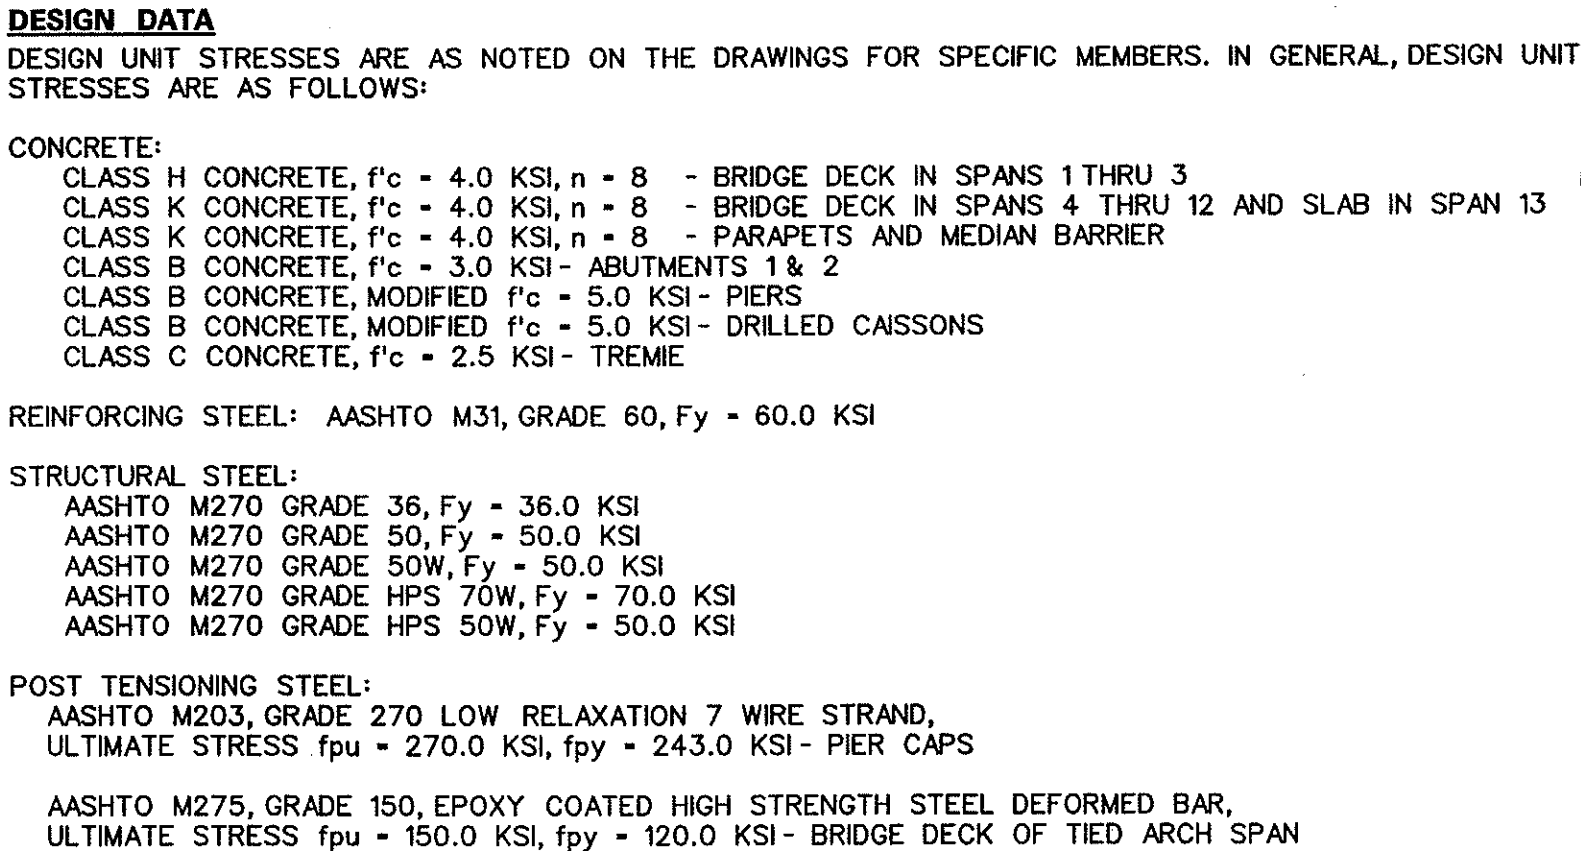
\includegraphics[width=0.65\textwidth]{overleaf/Appendix/Design drawings/Material design data.png}
    \caption{Material design data}
    \label{fig:materials}
\end{figure}
\begin{figure}[H]
    \centering
    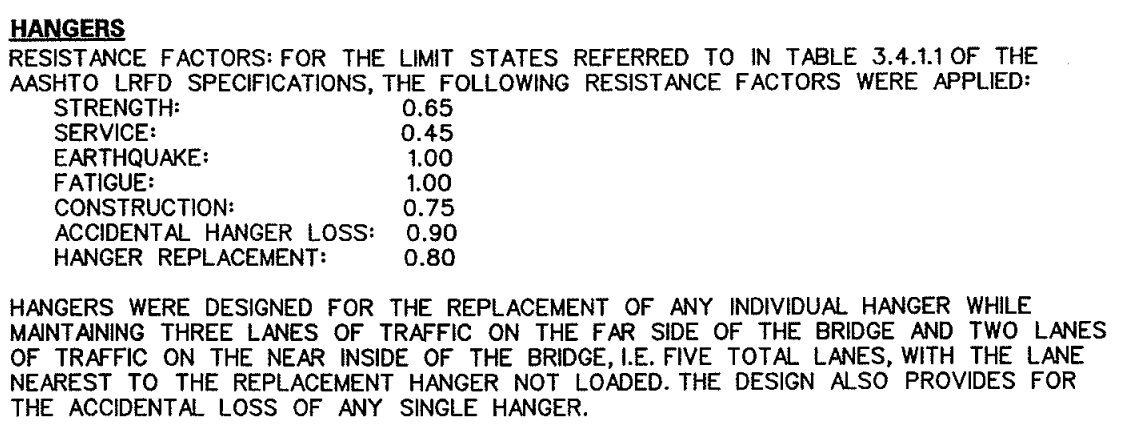
\includegraphics[trim={0 0.9cm 0 0cm},clip, width=0.6\textwidth]{overleaf/Appendix/Design drawings/Hanger resistance factor.PNG}
    \caption{Hanger resistance factors}
\end{figure}
\begin{figure}[H]
    \centering
    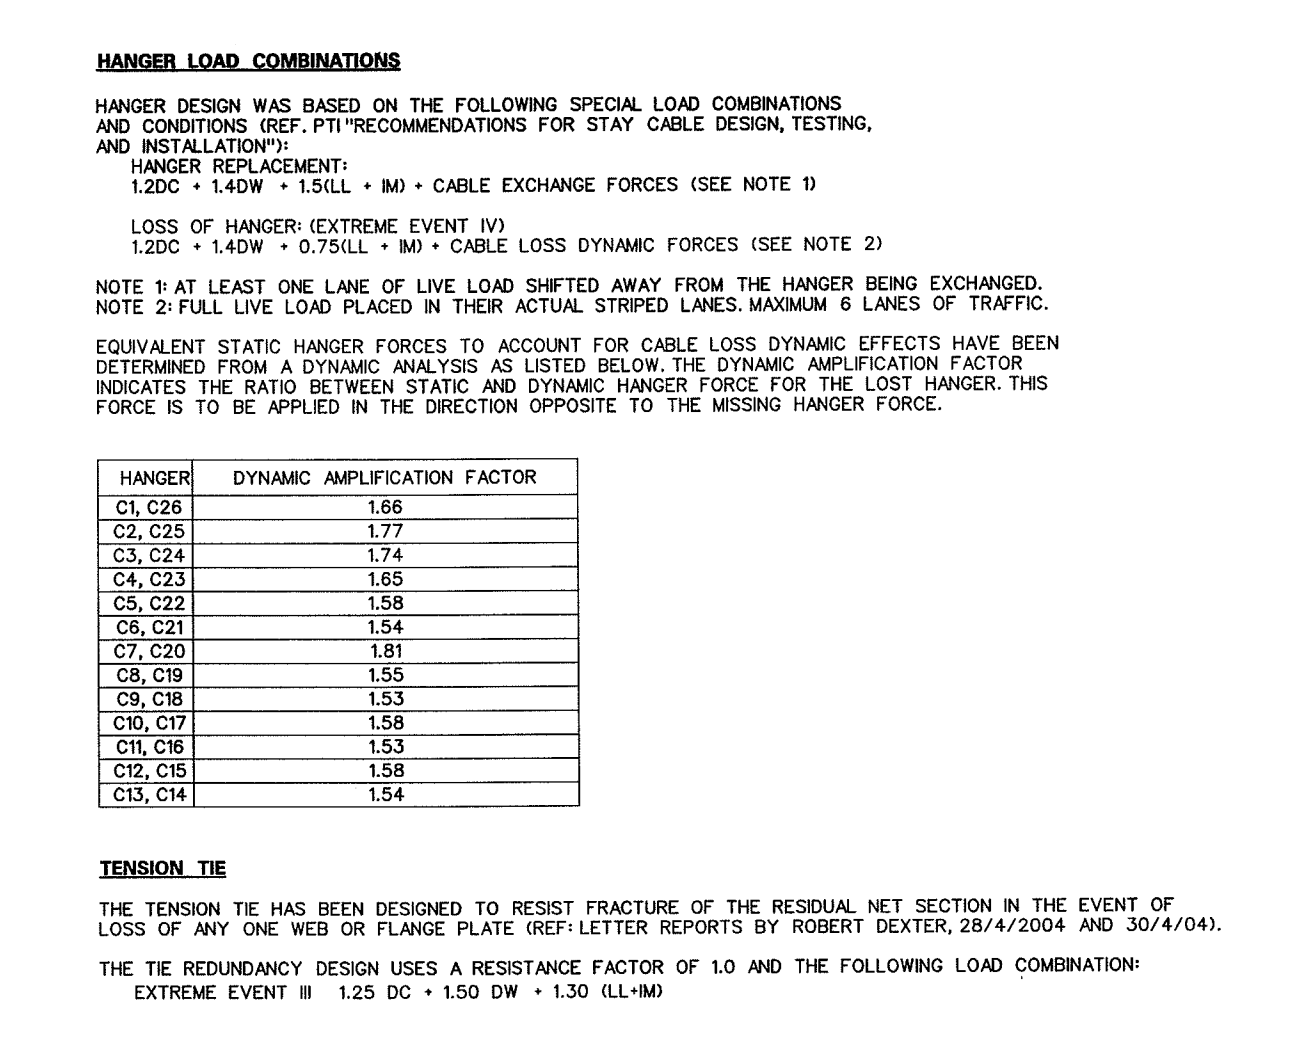
\includegraphics[trim={0 0.5cm 0 0.7cm},clip, width=0.69\textwidth]{overleaf/Appendix/Design drawings/Hanger load combination.png}
    \caption{Load combinations for extreme events and dynamic amplification factors}
    \label{fig:hanger_load_combination}
\end{figure}
%\begin{figure}[H]
%    \centering
%    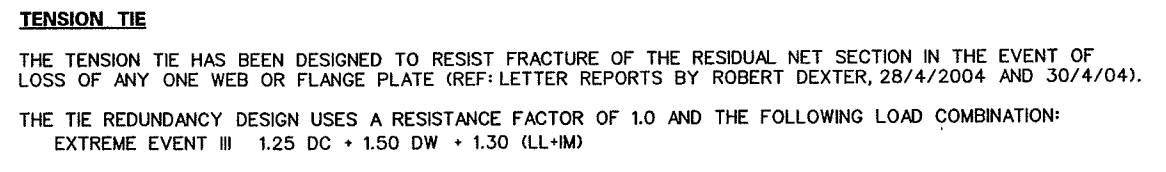
\includegraphics[width=0.8\textwidth]{overleaf/Appendix/Design drawings/Tension tie.PNG}
%    \caption{Tie fracture load combination}
%    \label{fig:tie_fracture_loads}
%\end{figure}

\section{Cross-sections} \label{app:cross_sections}
In this section, the cross-sections are introduced. The dimensions and the resistances were taken from the design verification tables, which are shown in Section \ref{app:design_verifications}. The materials of the cross-sections are adapted from the design data specified in Figure \ref{fig:materials}. The three characteristic cross-sections in the field are shown in Figures \ref{fig:cs_arch} to \ref{fig:cs_cable}. 

The cross-sectional properties for the arch rib, the tie girder and the cables are shown in Tables \ref{tab:cs_arch} to \ref{tab:cs_cable}.

\begin{table}[H]
\centering
\resizebox{0.85\textwidth}{!}{%
\begin{tabular}{lcccc}
\hline
Cross-Section          & Arch 1             & Arch 2             & Arch 3             &            \\ \hline
Flange width           & 1.219              & 1.219              & 1.219              & {[}m{]}    \\
Flange thickness       & 0.051              & 0.051              & 0.051              & {[}m{]}    \\
Subflange width        & 1.715              & 1.715              & 1.715              & {[}m{]}    \\
Subflange thickness    & 0.064              & 0.048              & 0.044              & {[}m{]}    \\
Web height             & 0.305              & 0.305              & 0.203              & {[}m{]}    \\
Web thickness          & 0.044              & 0.044              & 0.044              & {[}m{]}    \\ \hline
Area                   & 0.369              & 0.314              & 0.294              & {[}m$^2${]}   \\
Moment of intertia (z) & 0.150              & 0.137              & 0.134              & {[}m$^4${]}   \\
Moment of intertia (y) & 0.111              & 0.087              & 0.081              & {[}m$^4${]}   \\ \hline
Material               & Grade 270 HPS 70 W & Grade 270 HPS 70 W & Grade 270 HPS 50 W & {[}-{]}    \\
Yield strength         & 485                & 485                & 345                & {[}MPa{]}  \\
Young's modulus        & 210                & 210                & 210                & {[}GPa{]}  \\ \hline
Axial stiffness        & 77429              & 65997              & 61814              & {[}MN{]}   \\
Bending stiffness      & 31473              & 28673              & 28113              & {[}MNm$^2${]} \\
Weight                 & 2894.4             & 2467.0             & 2310.7             & {[}kg/m{]} \\ \hline
Normal resistance      & 130.0              & 108.8              & 82.3               & {[}MN{]}   \\
Moment resistance (z)  & 78.8               & 71.5               & 50.0               & {[}MNm{]}  \\
Moment resistance (y)  & 79.1               & 63.4               & 42.7               & {[}MNm{]}  \\ \hline
\end{tabular}
}
\caption{Cross-sectional properties of the arch rib segments}
\label{tab:cs_arch}
\end{table}
\begin{table}[H]
\centering
\resizebox{\textwidth}{!}{%
\begin{tabular}{lcccc}
\hline
Cross-Section          & Tie 1              & Tie 2              & Tie 3 - 4          &            \\ \hline
Flange width           & 1.359              & 1.327              & 1.314              & {[}m{]}    \\
Flange thickness       & 0.051              & 0.044              & 0.044              & {[}m{]}    \\
Subflange width        & 0.152              & 0.203              & 0.197              & {[}m{]}    \\
Subflange thickness    & 0.025              & 0.025              & 0.025              & {[}m{]}    \\
Web height             & 2.134              & 2.083              & 2.083              & {[}m{]}    \\
Web thickness          & 0.064              & 0.038              & 0.029              & {[}m{]}    \\ \hline
Area                   & 0.425              & 0.297              & 0.256              & {[}m$^2${]}   \\
Moment of intertia (z) & 0.293              & 0.220              & 0.204              & {[}m$^4${]}   \\
Moment of intertia (y) & 0.1341             & 0.0860             & 0.0695             & {[}m$^4${]}   \\ \hline
Material               & Grade 270 HPS 70 W & Grade 270 HPS 70 W & Grade 270 HPS 70 W & {[}-{]}    \\
Yield strength         & 485                & 485                & 485                & {[}MPa{]}  \\
Young's modulus        & 210                & 210                & 210                & {[}GPa{]}  \\ \hline
Axial stiffness        & 89148              & 62441              & 53736              & {[}MN{]}   \\
Bending stiffness      & 61596              & 46255              & 42811              & {[}MNm$^2${]} \\
Weight                 & 3332.4             & 2334.1             & 2008.7             & {[}kg/m{]} \\ \hline
Normal resistance      & 153.2              & 117.1              & 100.5              & {[}MN{]}   \\
Moment resistance (z)  & 100.8              & 82.8               & 76.2               & {[}MNm{]}  \\
Moment resistance (y)  & 76.2               & 56.6               & 45.8               & {[}MNm{]}  \\ \hline
\end{tabular}
}
\caption{Cross-sectional properties of the tie girder segments}
\label{tab:cs_tie}

\end{table}
\begin{table}[H]
\centering
\begin{tabular}{lcc}
\hline
Cross-Section          & Cable                                  &            \\ \hline
Strand diameter        & 15.2                                   & {[}mm{]}   \\
Strand area            & 140                                    & {[}mm$^2${]}  \\
Number of strands      & 29                                     & {[}-{]}    \\ \hline
Area                   & 0.0041                                 & {[}m$^2${]}   \\
Moment of intertia (z) & -                                      & {[}m$^4${]}   \\
Moment of intertia (y) & -                                      & {[}m$^4${]}   \\ \hline
Material               & Grade 270 Low Relaxation 7 Wire Strand & {[}-{]}    \\
Yield strength         & 1675                                   & {[}MPa{]}  \\
Young's modulus        & 196                                    & {[}GPa{]}  \\ \hline
Axial stiffness        & 796                                    & {[}MN{]}   \\
Bending stiffness      & -                                      & {[}MNm$^2${]} \\
Weight                 & 31.9                                   & {[}kg/m{]} \\ \hline
Normal resistance      & 6.8                                    & {[}MN{]}   \\
Moment resistance (z)  & -                                      & {[}MNm{]}  \\
Moment resistance (y)  & -                                      & {[}MNm{]}  \\ \hline
\end{tabular}

\caption{Cross-sectional properties of the cables}
\label{tab:cs_cable}
\end{table}

\newpage
\section{Weights} \label{app:weight}
The weights of the structural and non-structural components are estimated from the bridge and steel quantities presented in Fig. \ref{fig:bridge_quantities} and \ref{fig:steel_quantities}. The weights of the arch and the tie is assumed as their steel weights, including half of the anchorage weights for each. Also the upper lateral bracing is assigned to the arch. The weight of the deck is estimated from the concrete quantity and as well as the lower lateral bracing and the stringers. The weight of the utilities is taken as \SI{9388}{kN} fpr the total weight to correspond to the unfactored vertical reaction specified in the pot bearing data. The distributed weights are derived in Table  \ref{tab:weights}.

\begin{figure}[H]
    \centering
    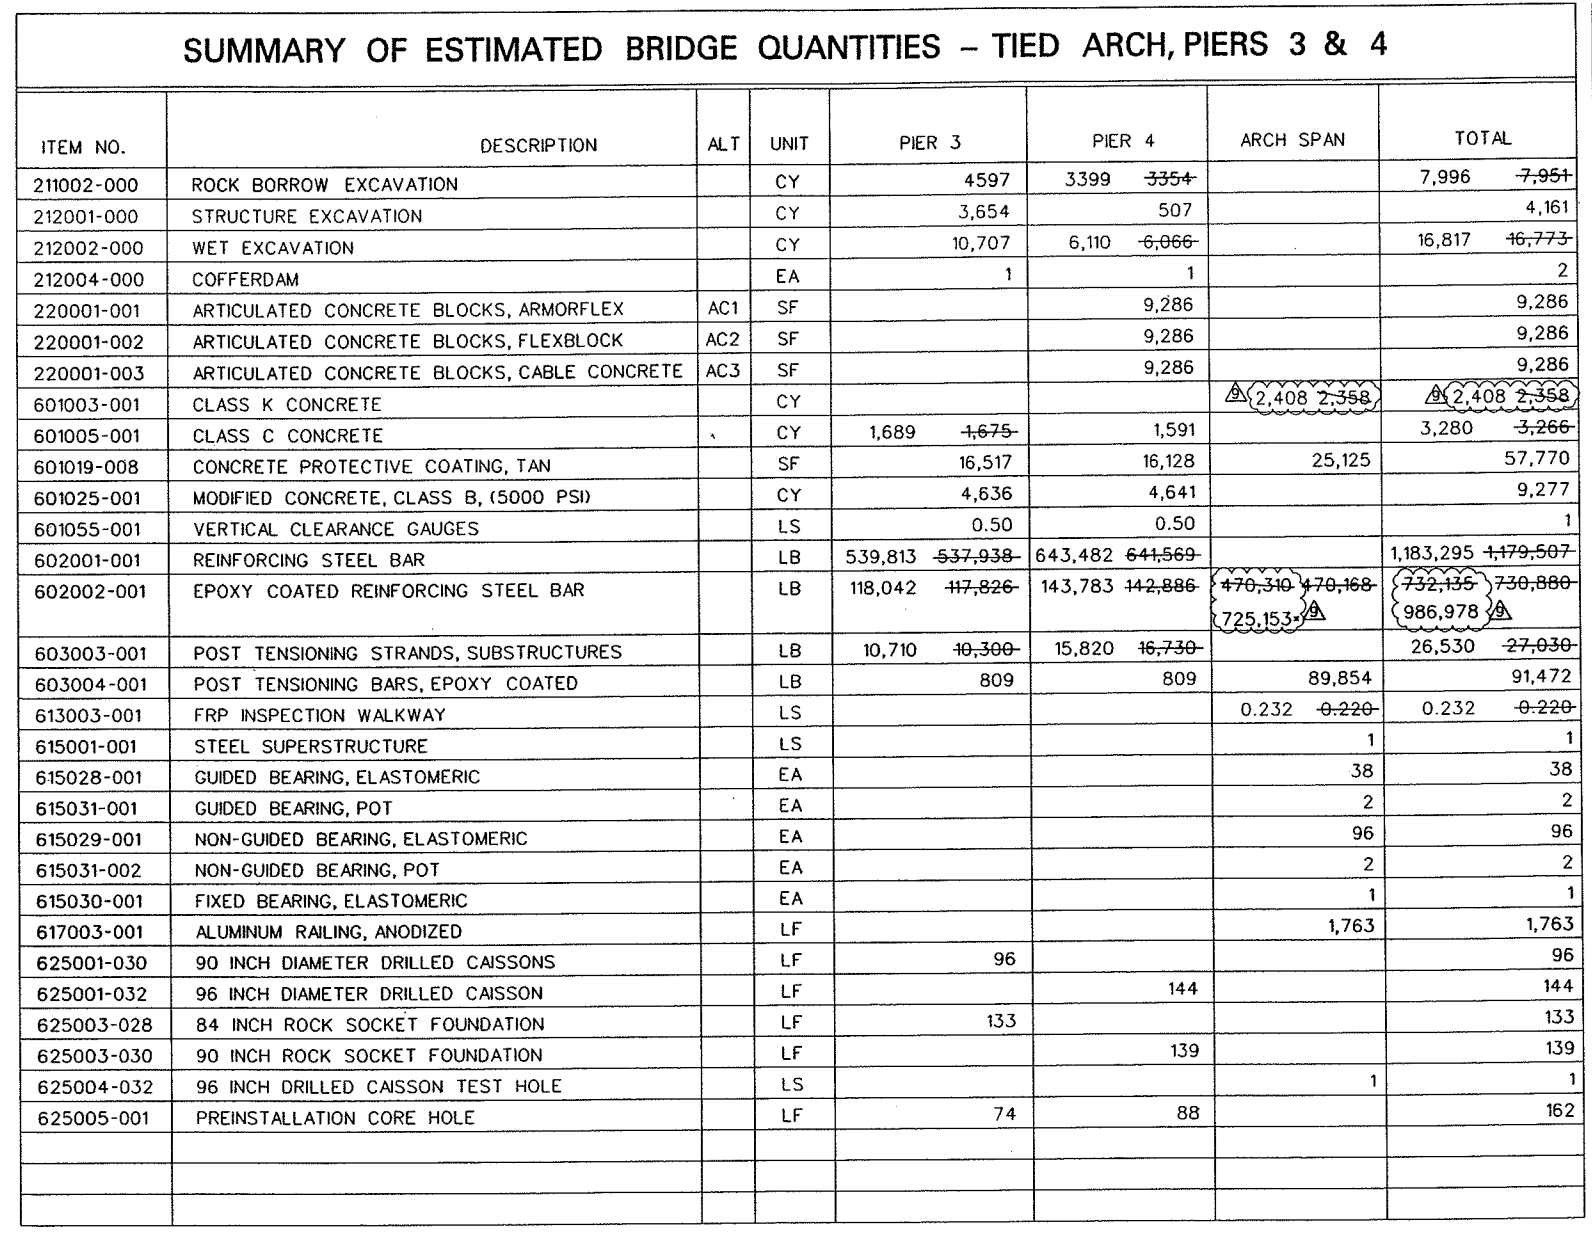
\includegraphics[trim={0 1.4cm 0 0},clip, width=0.55\textwidth]{overleaf/Appendix/Design drawings/estimated bridge quantities.PNG}
    \caption{Summary of estimated bridge quantities}
    \label{fig:bridge_quantities}
\end{figure}
\begin{figure}[H]
    \centering
    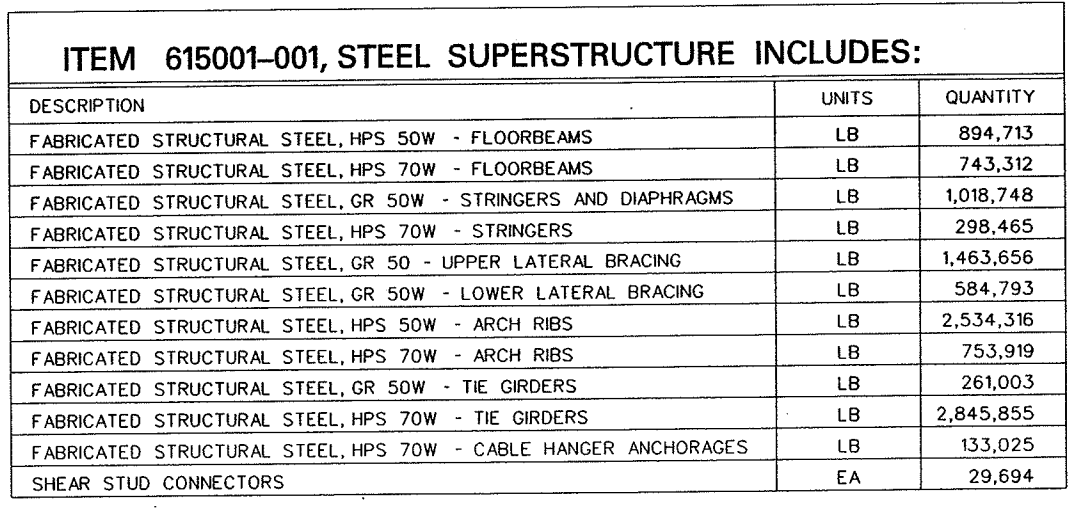
\includegraphics[trim={0 0cm 0 0.2cm},clip, width=0.5\textwidth]{overleaf/Appendix/Design drawings/Steel superstructure.PNG}
    \caption{Estimated steel quantities}
    \label{fig:steel_quantities}
\end{figure}

\begin{table}[H]
\centering
\caption{Estimated weights of the components}
\label{tab:weights}
\resizebox{0.55\textwidth}{!}{%
\begin{tabular}{lccc}
\toprule
Component & Total weight & Length  & Distributed weight \\
          & {[}kN{]}     & {[}m{]} & {[}kN/m{]}         \\ \midrule
Arch      & \SI{17524}{}        & 293.9   & 29.8               \\
Deck      & \SI{61776}{}        & 267.8   & 115.3              \\
Tie       & \SI{14116}{}        & 267.8   & 26.4               \\
Hangers   & \SI{401}{}          & \SI{1132}{}    & 0.35               \\
Utilities & \SI{9388}{}         & 267.8   & 35.1               \\
Total     & \SI{93817}{}        & 267.8   & 210.2              \\ \bottomrule
\end{tabular}
}
\end{table}

\section{Design verifications} \label{app:design_verifications}
The design verifications of the arch rib, the tie girder and the hangers are presented in Figs. \ref{fig:arch_design_verification} to \ref{fig:hanger_design_verification}.
\begin{figure}[H]
    \centering
    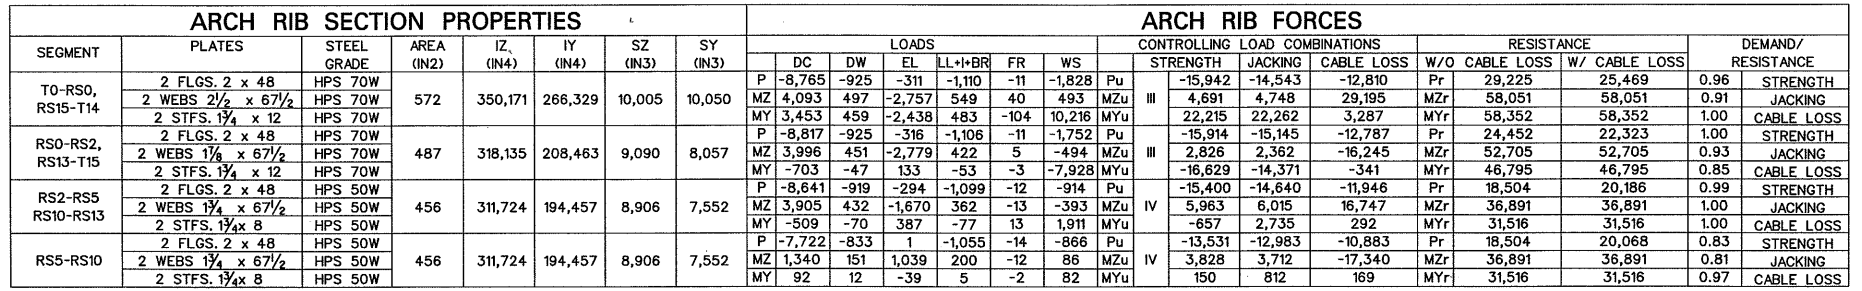
\includegraphics[width=\textwidth]{overleaf/Appendix/Design drawings/arch rib verifications.PNG}
    \caption{Design verifications of the arch rib segments}
    \label{fig:arch_design_verification}
\end{figure}
\begin{figure}[H]
    \centering
    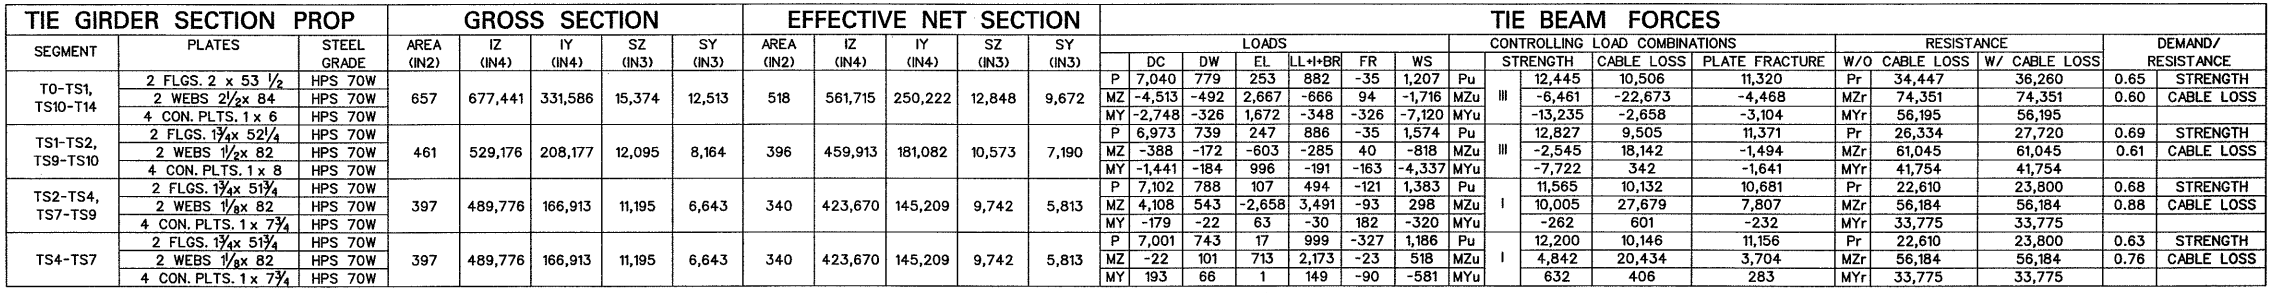
\includegraphics[width=\textwidth]{overleaf/Appendix/Design drawings/tie girder verifications.PNG}
    \caption{Design verifications of the tie girder segments}
    \label{fig:tie_design_verification}
\end{figure}
\begin{figure}[H]
    \centering
    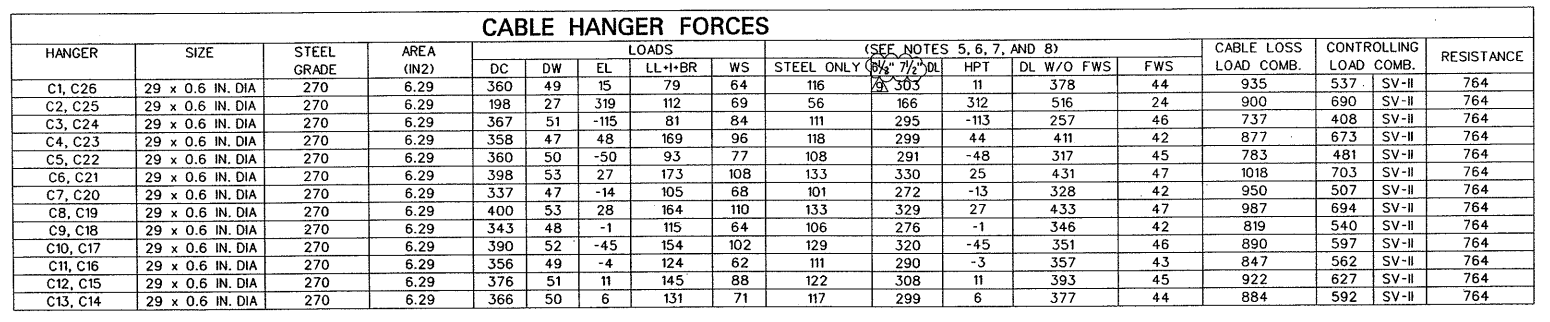
\includegraphics[width=\textwidth]{overleaf/Appendix/Design drawings/cable verifications.PNG}
    \caption{Design verifications of the hangers}
    \label{fig:hanger_design_verification}
\end{figure}



\newpage
\chapter{Model}
\label{AppendixModel}
\section{Hangers}
\label{Appendix_A_Hangers}
In this section, the non-linear effects of the hangers are considered. Assuming a parabolic displacement curve, the secondary effects are approximated by Eq. \eqref{eq:cable}, which gives the cable elongation $\delta$ at a stress of $\sigma_2$. Where $a$ is the horizontal component of the cable length $c$ at a stress of $\sigma_1$, $E$ is the modulus of elasticity and $\gamma$ is the weight of the cable \cite{NIELS}. 

\begin{equation}
    \frac{\delta}{c}= \frac{\sigma_2-\sigma_1}{E} 
    + \frac{\gamma^2\,c^2}{24}\,\left(\frac{1}{\sigma_1^2} -\frac{1}{\sigma_2^2} \right) 
    + \frac{\gamma^2\,c^2}{12\,E}\,\left(\frac{1}{\sigma_2} -\frac{1}{\sigma_1} \right)
    \label{eq:cable}
\end{equation}

To judge the influence on the Blennerhassett Island Bridge, the following values are assumed: $a=\SI{26}{m}$, $c=\SI{59.5}{m}$, $E=\SI{196}{GPa}$, $\gamma=\SI{78.5}{kN/m^3}$ and $\sigma_1=0.45\,f_y=\SI{750}{MPa}$. The elongation of the cable is compared to the assumed linear elastic behaviour of a rod, which is shown in Fig. \ref{fig:hanger_approximation}.

\begin{figure}[H]
    \centering
    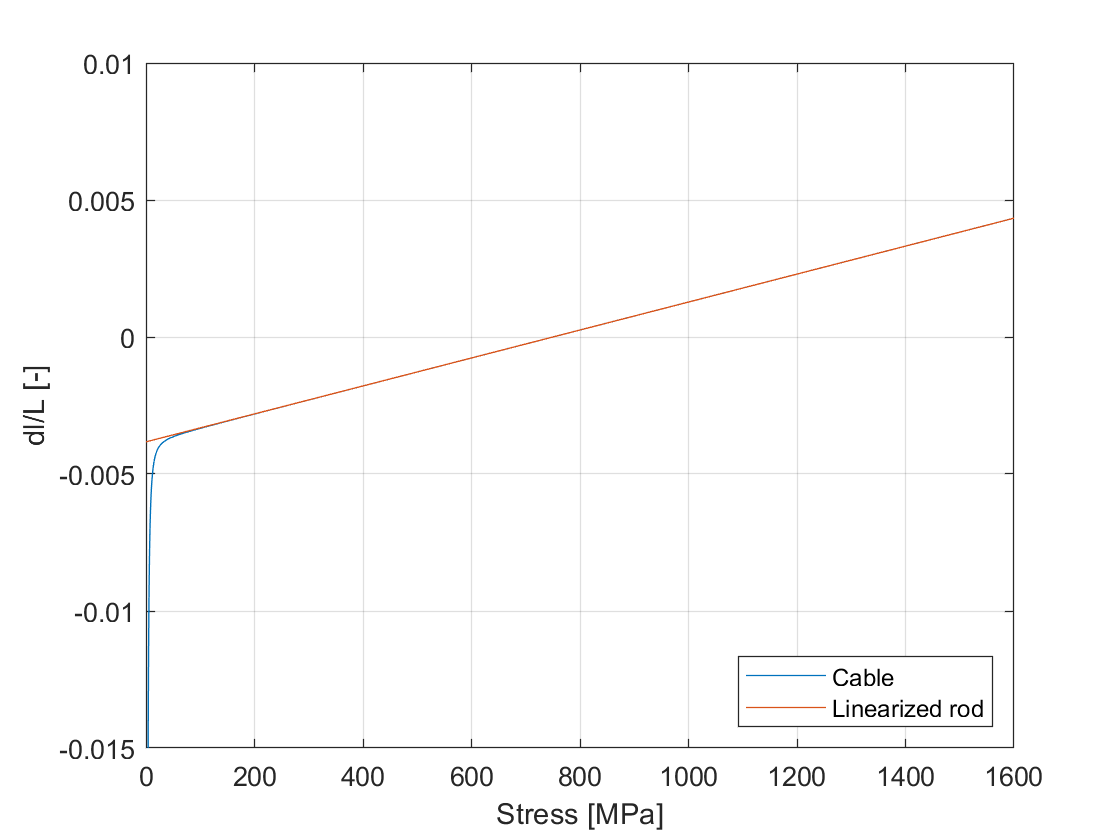
\includegraphics[width=0.7\textwidth]{overleaf/Appendix/Pictures/hanger_approximation.png}
    \caption{Cable elongation considering secondary effects}
    \label{fig:hanger_approximation}
\end{figure}

Only for cables stresses below \SI{100}{MPa}, which corresponds to 6\% of its yield stress, secondary effects become relevant. As stresses in this range are not occurring in any calculation, secondary effects can be neglected.

\newpage
\section{Live loading} \label{Appendix_Liveloading}
In this section, the arrangement of the live loads on the deck is investigated. The three design states strength, cable replacement and cable loss are treated individually as different circumstances apply. The live load relevant for fatigue can then be derived from the strength limit state. In the first step, the location of each lane is defined. According to the AASHTO design provisions, the width of every lane is equal to $\SI{12}{ft} = \SI{3.7}{m}$ of which \SI{3}{m} are loaded and the center of the applied forces $x_c$ can be derived \cite{AASHTO}. The force applied to the tie girder $F_r$ can then be calculated according to Eq. \ref{eq:reaction} using the width of the deck $w_{deck}=\SI{107}{ft}=\SI{32.6}{m}$.
\begin{equation}
    F_r = \frac{x_c}{w_{deck}}
    \label{eq:reaction}
\end{equation}
In a second step, the amount of loaded lanes under the consideration of the multiple presence factor (MPF) is determined. As the multiple presence factor decreases with the number of loaded lanes, each possibility is calculated to find the worst arrangement. The calculations are conducted for a unit lane load. The obtained factor relates the load on each lane to the load applied to the investigated tie girder. The factor can then be used for the calculation of the force on the tie of the distributed lane load ($q_{LL}=\SI{9.3}{kN/m}$) as well as of the design truck load ($Q_{LL}=\SI{325}{kN}$). For the design truck load, an additional dynamic multiplier of 1.33 is taken into account. 

\subsection*{Vehicular use} \label{Appendx_A_Live_loading_1}
In the first strength limit state, the entire width of the deck is available to traffic. The lanes are arranged as densely to one side as possible with the first lane starting at $\SI{4.6}{ft}=\SI{1.4}{m}$ from the investigated arch plane. The calculations presented in Table \ref{tab:app_ll_uls} show that the worst arrangement results with six loaded lanes. 

\begin{table}[H]
\centering
\begin{tabular}{cccccccccccc}
\cline{2-11}
             & Lane     &  & 1    & 2    & 3    & 4    & 5    & 6    & 7    & 8    &      \\
             & Centroid &  & 2.9  & 6.6  & 10.2 & 13.9 & 17.5 & 21.2 & 24.8 & 28.5 &      \\
             & Reaction &  & 0.91 & 0.80 & 0.69 & 0.57 & 0.46 & 0.35 & 0.24 & 0.13 &      \\ \hline
Loaded Lanes & MPF      &  &      &      &      &      &      &      &      &      & Sum  \\ \hline
1            & 1.2      &  & 1.09 &      &      &      &      &      &      &      & 1.09 \\
2            & 1.0      &  & 0.91 & 0.80 &      &      &      &      &      &      & 1.71 \\
3            & 0.85     &  & 0.77 & 0.68 & 0.58 &      &      &      &      &      & 2.04 \\
4            & 0.75     &  & 0.68 & 0.60 & 0.52 & 0.43 &      &      &      &      & 2.23 \\
5            & 0.70     &  & 0.64 & 0.56 & 0.48 & 0.40 & 0.32 &      &      &      & 2.40 \\
6            & 0.65     &  & 0.59 & 0.52 & 0.45 & 0.37 & 0.30 & 0.23 &      &      & 2.46 \\
7            & 0.60     &  & 0.55 & 0.48 & 0.41 & 0.34 & 0.28 & 0.21 & 0.14 &      & 2.41 \\
8            & 0.55     &  & 0.50 & 0.44 & 0.38 & 0.32 & 0.25 & 0.19 & 0.13 & 0.07 & 2.28 \\ \hline
\end{tabular}
\caption{Force on tie girder for ultimate limit state under unit lane load}
\label{tab:app_ll_uls}
\end{table}

Six loaded lanes yield a factor of 2.46. Hence the load applied on the investigated arch plane can be calculated according to Eqs. \eqref{eq:q_ll_uls} and \eqref{eq:Q_ll_uls}. The decisive arrangement is illustrated in Fig. \ref{fig:app_hangers_uls}.
\begin{equation}
    q_{ll, uls} = 2.46 \cdot \SI{9.3}{kN/m} = \SI{22.9}{kN/m}
    \label{eq:q_ll_uls}
\end{equation}
\begin{equation}
    Q_{ll, uls} = 2.46 \cdot 1.33 \cdot \SI{325}{kN} = \SI{1063}{kN}
    \label{eq:Q_ll_uls}
\end{equation}

\begin{figure}[H]
    \centering
    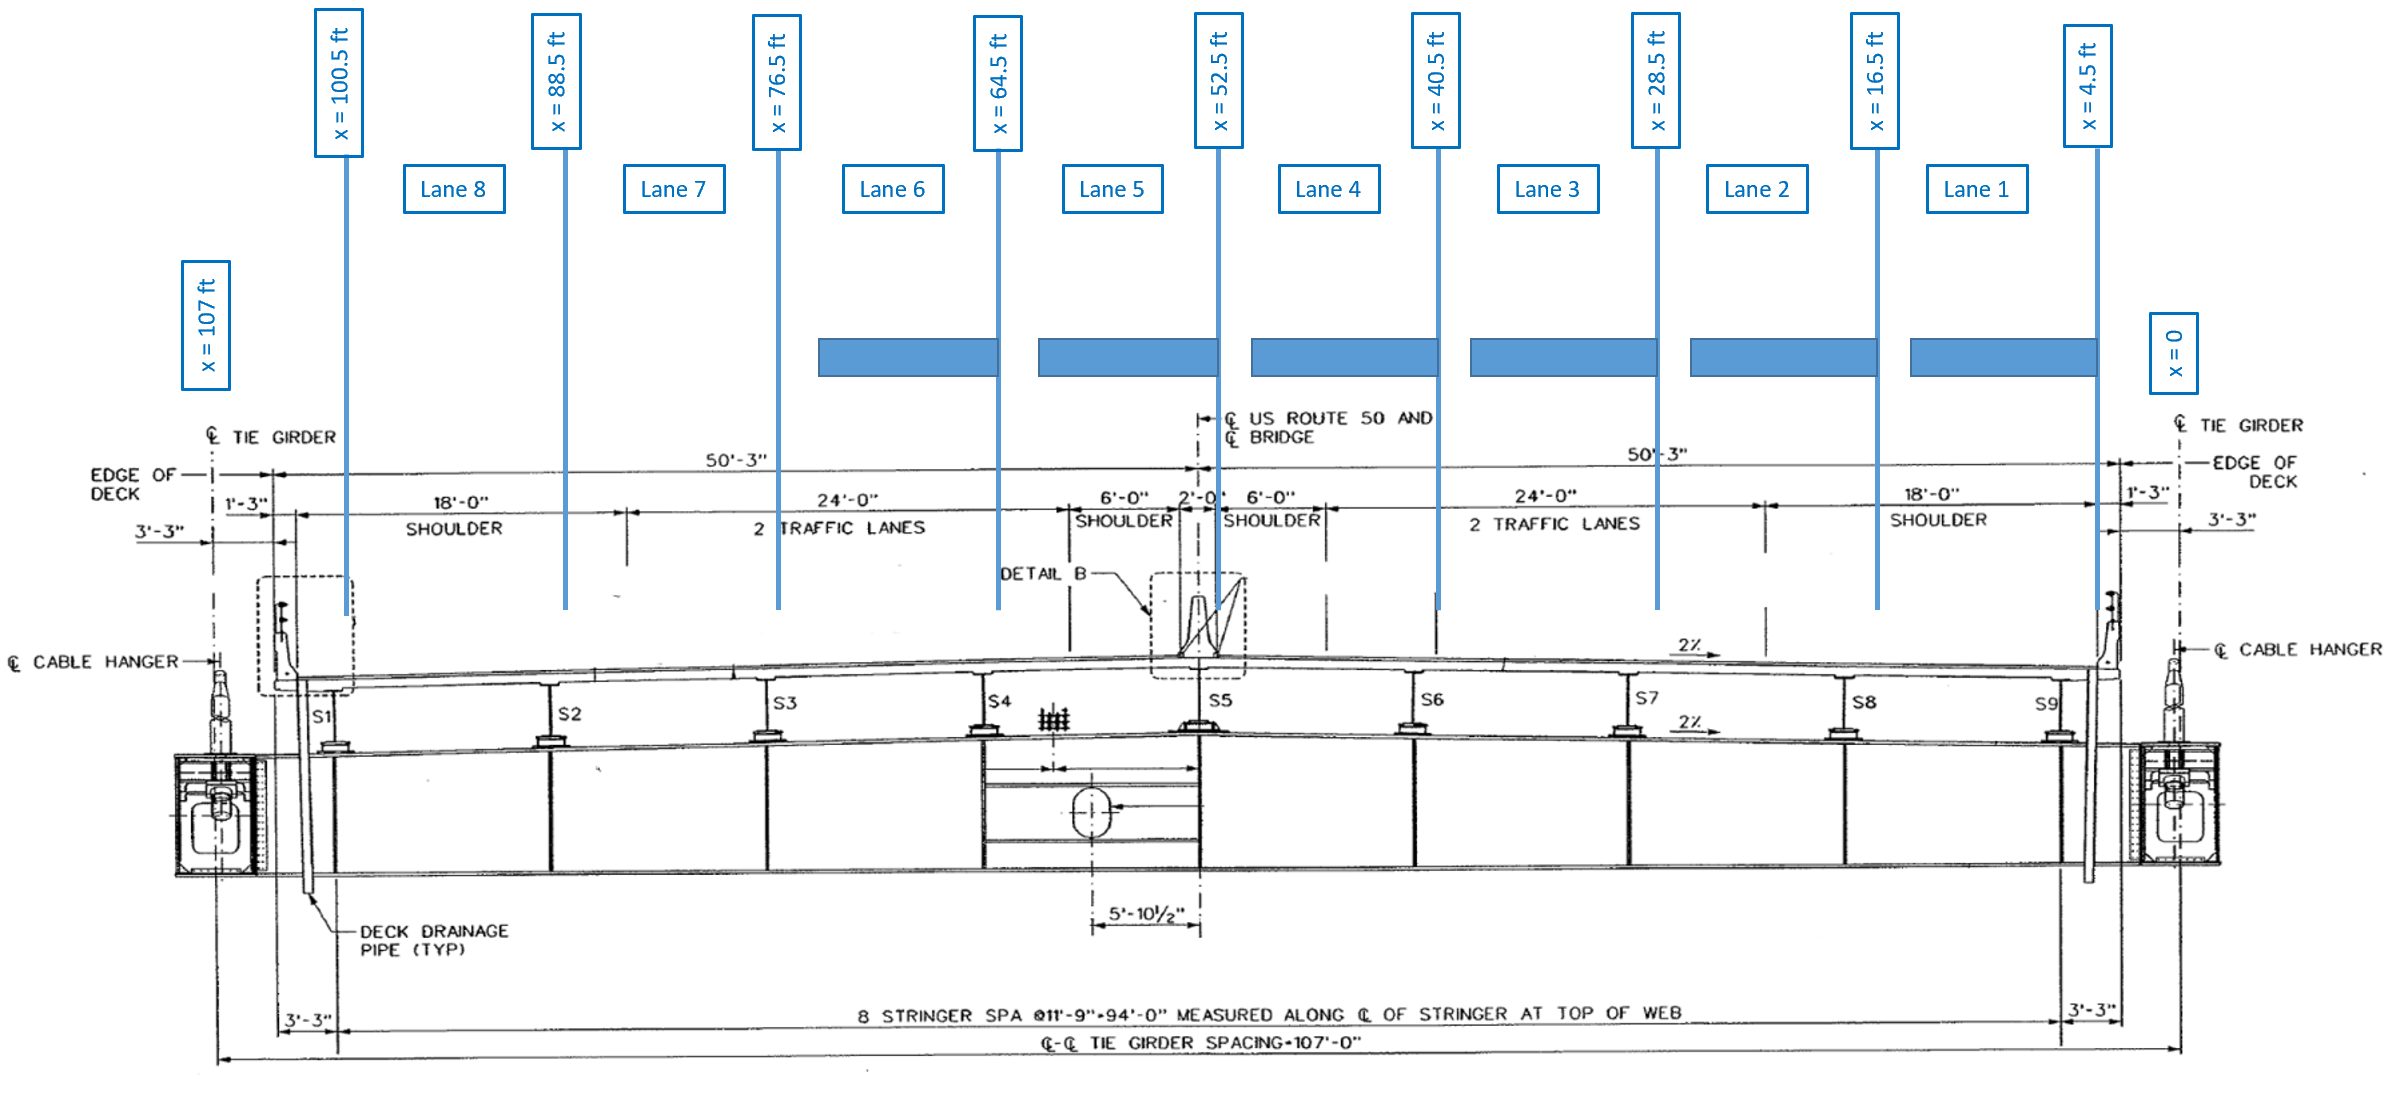
\includegraphics[width=\textwidth]{overleaf/Appendix/Pictures/Cross_Section_LL_ULS.PNG}
    \caption{Live load arrangement in the strength limit state}
    \label{fig:app_hangers_uls}
\end{figure}


\subsection*{Fatigue} \label{Appendx_A_Live_loading_15}
The fatigue limit state is investigated according to the recommendations for stay cable design, testing and installation by the Post Tensioning Institute (PTI). The corresponding loading is composed of a single design truck which occupies the lane resulting in the highest effect on the investigated stay cable \cite{PTI}. It corresponds to the lane closest to the border in this case, for which, according to Table \ref{tab:app_ll_uls}, the force on the tie girder is equal to 91\% of the design truck load. It results in the fatigue load according to Eq. \ref{eq:Q_fat}.

\begin{equation}
    Q_{fat} = 0.91 \cdot \SI{325}{kN} = \SI{296}{kN}
    \label{eq:Q_fat}
\end{equation}

\subsection*{Cable replacement} \label{Appendx_A_Live_loading_2}
In the event of cable replacement, one lane is shifted away from the hanger being exchanged. Besides that, the lanes are located at the same positions as in the ultimate limit state. A load for the replacement truck is disregarded for in this investigation. The calculation of the different arrangements is presented in Table \ref{tab:app_ll_hanger_replacement}.
\begin{table}[H]
\centering
\caption{Force on tie girder for hanger replacement under unit lane load}
\label{tab:app_ll_hanger_replacement}
\resizebox{.8\textwidth}{!}{%
\begin{tabular}{cccccccccccc}
\cline{2-11}
             & Lane     &  & 1    & 2    & 3    & 4    & 5    & 6    & 7    & 8    &      \\
             & Centroid &  & 2.9  & 6.6  & 10.2 & 13.9 & 17.5 & 21.2 & 24.8 & 28.5 &      \\
             & Reaction &  & 0.91 & 0.80 & 0.69 & 0.57 & 0.46 & 0.35 & 0.24 & 0.13 &      \\ \hline
Loaded Lanes & MPF      &  &      &      &      &      &      &      &      &      & Sum  \\ \hline
1            & 1.2      &  & -    & 0.96 &      &      &      &      &      &      & 0.96 \\
2            & 1.0      &  & -    & 0.80 & 0.69 &      &      &      &      &      & 1.49 \\
3            & 0.85     &  & -    & 0.68 & 0.58 & 0.49 &      &      &      &      & 1.75 \\
4            & 0.75     &  & -    & 0.60 & 0.52 & 0.43 & 0.35 &      &      &      & 1.89 \\
5            & 0.70     &  & -    & 0.56 & 0.48 & 0.40 & 0.32 & 0.25 &      &      & 2.01 \\
6            & 0.65     &  & -    & 0.52 & 0.45 & 0.37 & 0.30 & 0.23 & 0.15 &      & 2.02 \\
7            & 0.60     &  & -    & 0.48 & 0.41 & 0.34 & 0.28 & 0.21 & 0.14 & 0.08 & 1.94 \\ \hline
\end{tabular}
}
\end{table}

The resulting loads on the investigated arch plane are presented in Eqs. \eqref{eq:q_ll_repl} and \eqref{eq:Q_ll_repl}.
\begin{equation}
    q_{ll, repl} = 2.02 \cdot \SI{9.3}{kN/m} = \SI{18.8}{kN/m}
    \label{eq:q_ll_repl}
\end{equation}
\begin{equation}
    Q_{ll, repl} = 2.02 \cdot 1.33 \cdot \SI{325}{kN} = \SI{874}{kN}
    \label{eq:Q_ll_repl}
\end{equation}

\subsection*{Cable loss} \label{Appendx_A_Live_loading_3}
In the extreme event of cable loss, not the deck's entire width is available to the live loads. For this case, only the four actual marked lanes are available. Their locations were taken from the design drawings. The investigation in Table \ref{tab:app_ll_cable_loss} shows that all of these lanes are loaded in the worst arrangement.
\begin{table}[H]
\centering
\caption{Force on tie girder for cable loss under unit lane load}
\label{tab:app_ll_cable_loss}
\begin{tabular}{cccccccc}
\cline{2-7}
             & Lane     &  & 1    & 2    & 3    & 4    &      \\
             & Centroid &  & 8.4  & 12.0 & 20.0 & 23.6 &      \\
             & Reaction &  & 0.74 & 0.63 & 0.39 & 0.28 &      \\ \hline
Loaded Lanes & MPF      &  &      &      &      &      & Sum  \\ \hline
1            & 1.2      &  & 0.89 &      &      &      & 0.89 \\
2            & 1.0      &  & 0.74 & 0.63 &      &      & 1.37 \\
3            & 0.85     &  & 0.63 & 0.54 & 0.33 &      & 1.50 \\
4            & 0.75     &  & 0.56 & 0.47 & 0.29 & 0.21 & 1.53 \\ \hline
\end{tabular}
\end{table}

The loads resulting on the tie girder are calculated in Eqs. \eqref{eq:q_ll_loss} and \eqref{eq:Q_ll_loss}.
\begin{equation}
    q_{ll, loss} = 1.53 \cdot \SI{9.3}{kN/m} = \SI{14.2}{kN/m}
    \label{eq:q_ll_loss}
\end{equation}
\begin{equation}
    Q_{ll, loss} = 1.42 \cdot 1.33 \cdot \SI{325}{kN} = \SI{660}{kN}
    \label{eq:Q_ll_loss}
\end{equation}

An illustration of the load arrangement for the event of cable loss is presented in Fig. \ref{fig:app_hangers_cable_loss}.

\begin{figure}[H]
    \centering
    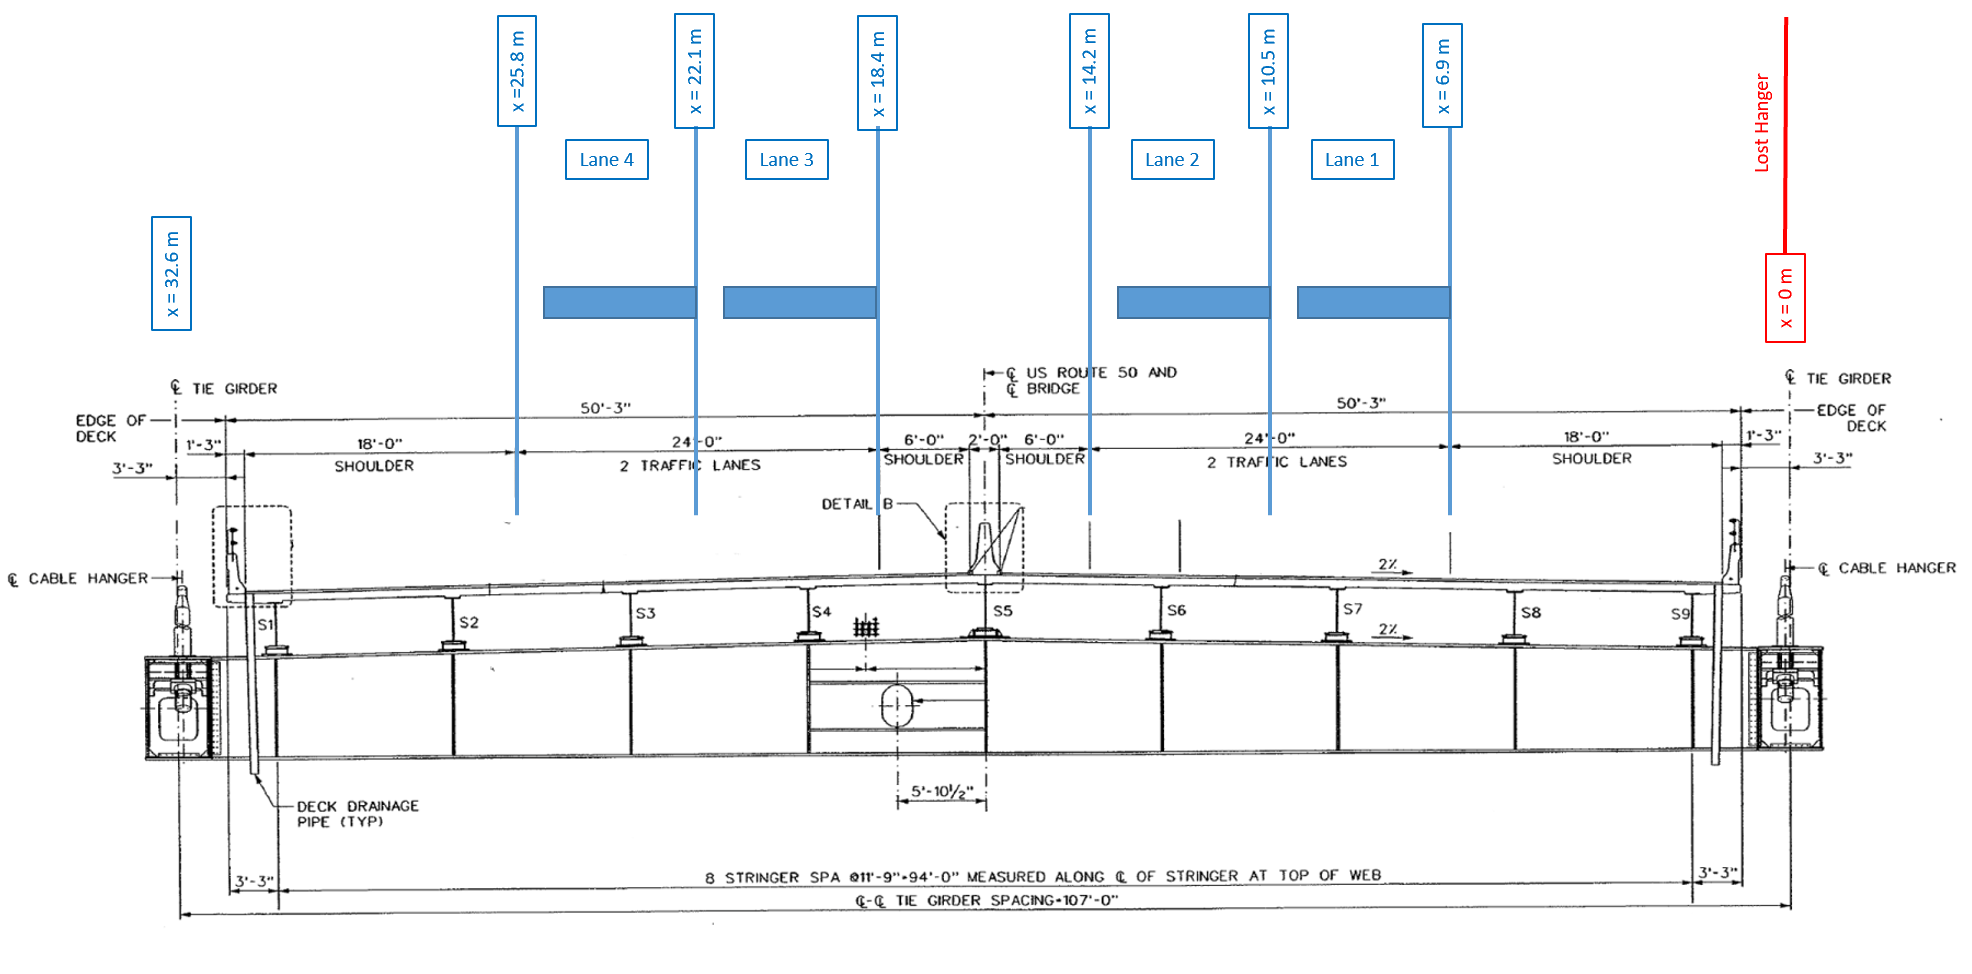
\includegraphics[width=\textwidth]{overleaf/Appendix/Pictures/Cross_Section_LL_Cable Loss.PNG}
    \caption{Live load arrangement for cable loss}
    \label{fig:app_hangers_cable_loss}
\end{figure}

\newpage
\section{Verification} \label{app:model_verification}
The model is verified by comparing it to the model of a parallel Master Thesis by Moritz Studer. For the comparison, the elastic response under the dead loading is compared. The two responses are shown in Figures \ref{fig:verification_1} and \ref{fig:verification_2} respsectively.

\begin{figure}[H]
    \centering
    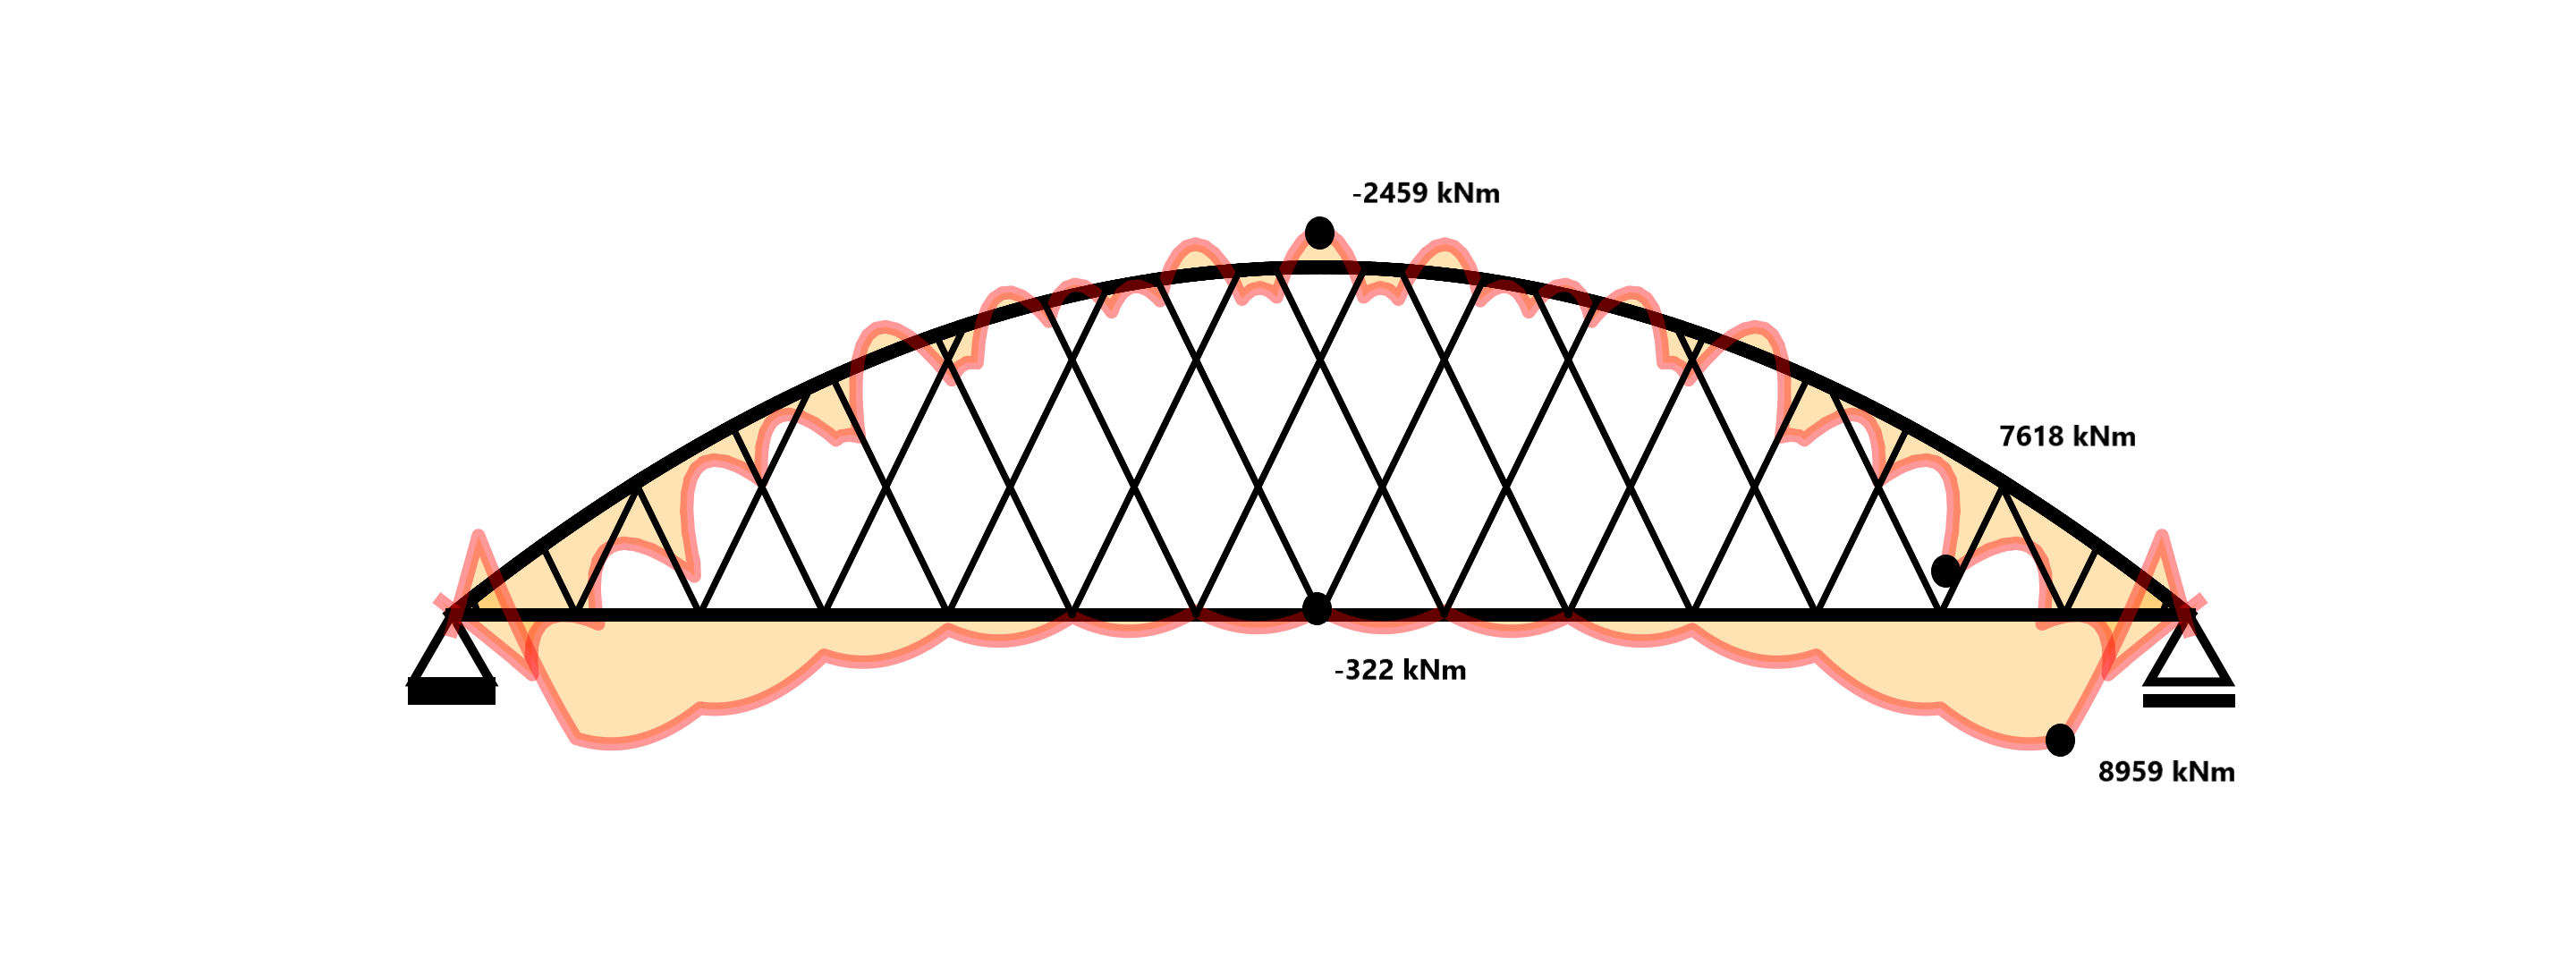
\includegraphics[trim={12cm 5cm 10cm 5cm},clip, width=\textwidth]{calculations/model comparison/dead_load.png}
    \caption{Elastic response for dead loading in the model of this Thesis}
    \label{fig:verification_1}
\end{figure}

\begin{figure}[H]
    \centering
    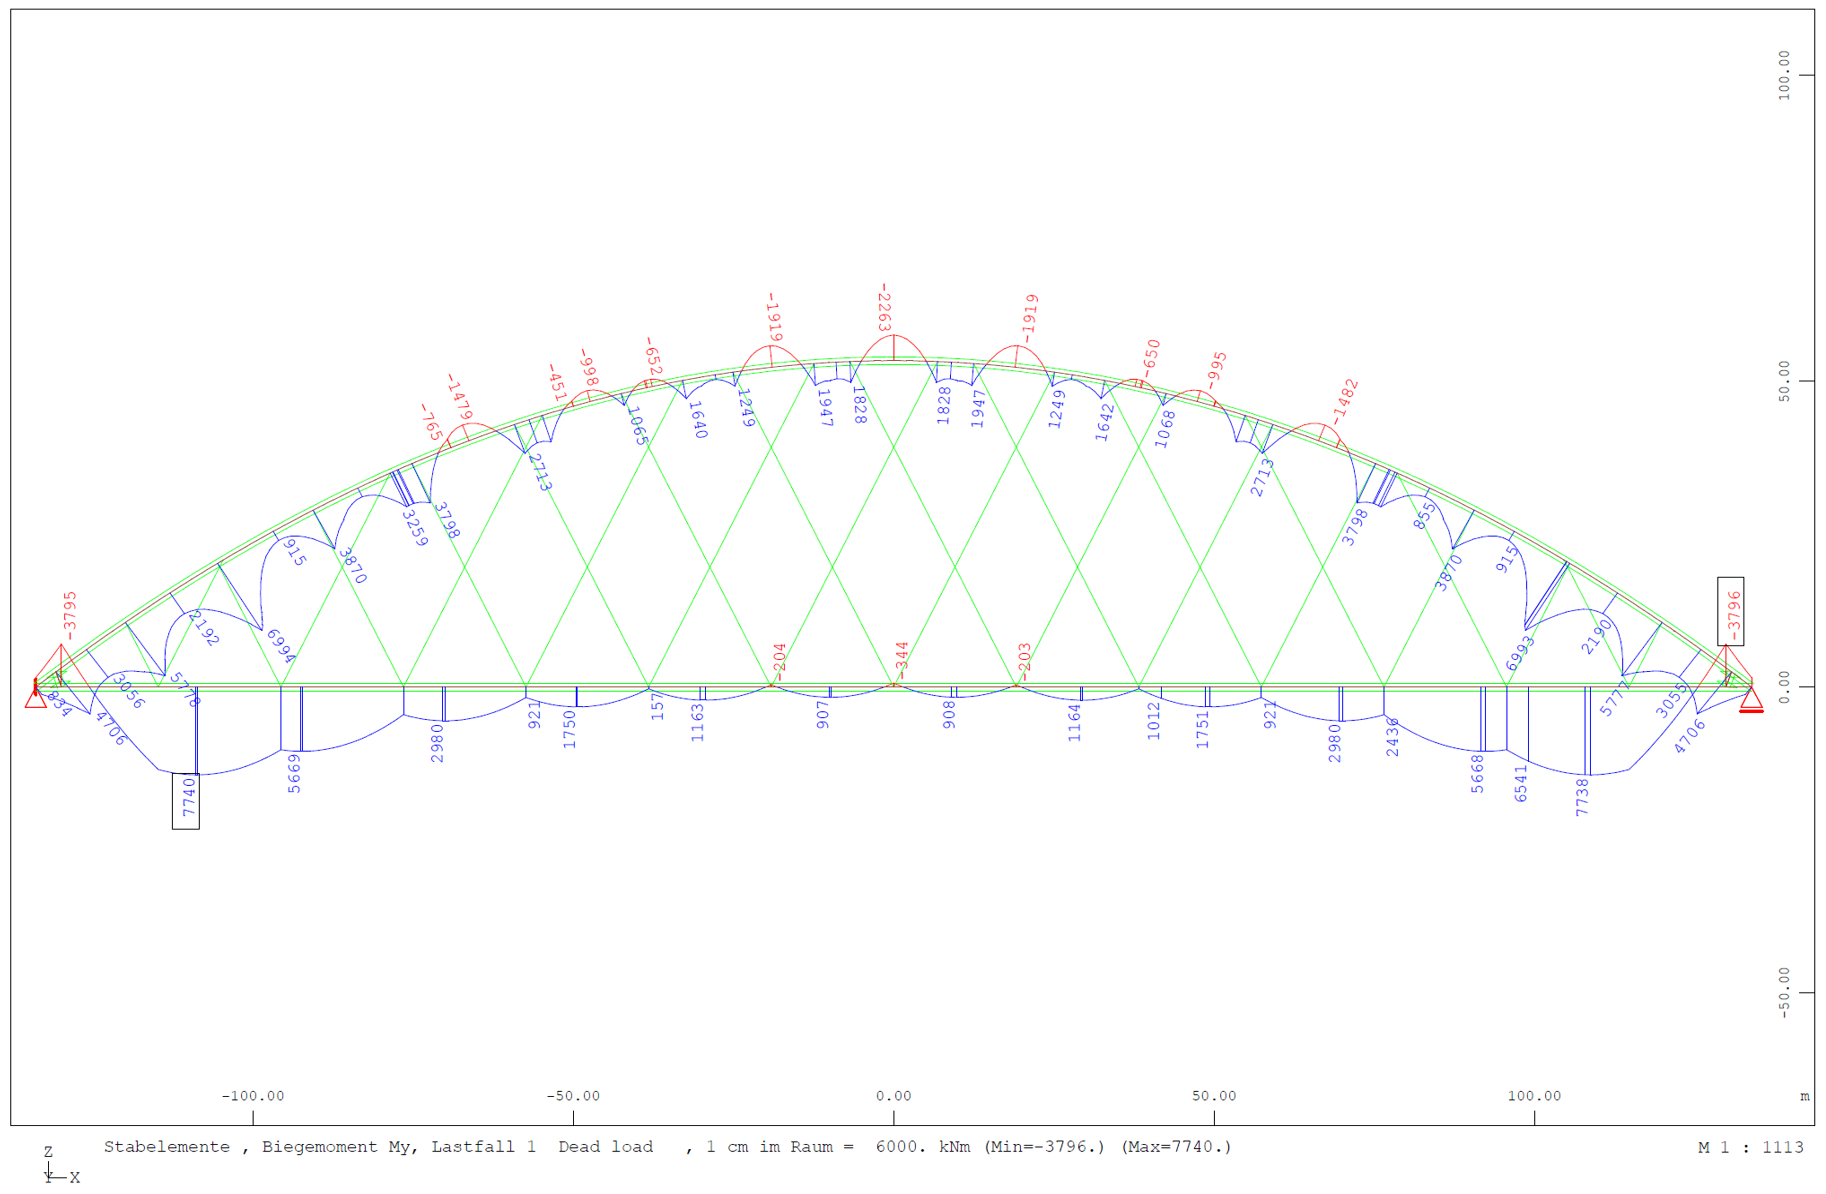
\includegraphics[trim={0.3cm 4cm 0.8cm 3.5cm},clip, width=\textwidth]{calculations/model comparison/dead_load_comparison.PNG}
    \caption{Elastic response for dead loading in the model of a parallel Thesis}
    \label{fig:verification_2}
\end{figure}

The responses in the two models qualitatively agree well. Both of them indicate the strongest moments in the arch and the tie near the knuckle. The respective moments of in the arch are \SI{7618}{kNm} in the used model and \SI{6993}{kNm} in the comparative model. For the tie, the difference is slightly larger at \SI{8959}{kNm} and \SI{7738}{kNm}. The generally larger moment magnitudes in the model of this Thesis can be explained by the assumption of higher dead loads. However, as the distributions visually agree very well, the model is considered to be verified.


\chapter{Cost estimation}
In this chapter, the hanger unit costs are derived. The unit costs for the free length, the detailing and installation and the anchorages were received from a partner in the industry for \SI{150}{mm^2} strands and are given in Table \ref{tab:hanger_unit}.

\begin{table}[H]
\centering
\begin{tabular}{ccc}
\hline
Free length      & Detailing and installation & Anchorages    \\
3.00 \$/strand/m & 12.5 \$/strand/m           & 185 \$/strand \\ \hline
\end{tabular}
\caption{Hanger unit costs}
\label{tab:hanger_unit}
\end{table}

The total costs are calculated in Table \ref{tab:hanger_costs} for a single hanger set of the Blennerhassett Island Bridge. 

\begin{table}[H]
\centering
\resizebox{\textwidth}{!}{%
\begin{tabular}{lcccccc}
\hline
Hanger & Length  & Number of strands & Free length & Anchorage & Detailing and installation & Total cost \\
       & {[}m{]} & {[}-{]}           & {[}\${]}         & {[}\${]}       & {[}\${]}                   & {[}\${]}   \\ \hline
T1-H1  & 10.8    & 29                & \SI{938}{}              & \SI{5365}{}           & \SI{3907}{}                       & \SI{10210}{}      \\
T2-H2  & 21.5    & 29                & \SI{1868}{}             & \SI{5365}{}           & \SI{7784}{}                       & \SI{15017}{}      \\
T1-H3  & 24.1    & 29                & \SI{2097}{}             & \SI{5365}{}           & \SI{8738}{}                       & \SI{16201}{}      \\
T3-H4  & 31.3    & 29                & \SI{2721}{}             & \SI{5365}{}           & \SI{11339}{}                      & \SI{19425}{}      \\
T2-H5  & 38.3    & 29                & \SI{3332}{}             & \SI{5365}{}           & \SI{13882}{}                      & \SI{22579}{}      \\
T4-H6  & 39.8    & 29                & \SI{3461}{}             & \SI{5365}{}           & \SI{14421}{}                      & \SI{23247}{}      \\
TS-H7  & 46.9    & 29                & \SI{4083}{}             & \SI{5365}{}           & \SI{17012}{}                      & \SI{26460}{}      \\
T3-H8  & 48.8    & 29                & \SI{4245}{}             & \SI{5365}{}           & \SI{17686}{}                      & \SI{27295}{}      \\
T6-H9  & 52.6    & 29                & \SI{4574}{}             & \SI{5365}{}           & \SI{19059}{}                      & \SI{28998}{}      \\
T4-H10 & 55.1    & 29                & \SI{4797}{}             & \SI{5365}{}           & \SI{19986}{}                      & \SI{30147}{}      \\
T7-H11 & 56.5    & 29                & \SI{4917}{}             & \SI{5365}{}           & \SI{20488}{}                      & \SI{30770}{}      \\
TS-H12 & 58.2    & 29                & \SI{5061}{}             & \SI{5365}{}           & \SI{21087}{}                      & \SI{31512}{}      \\
T8-H13 & 58.5    & 29                & \SI{5088}{}             & \SI{5365}{}           & \SI{21201}{}                      & \SI{31654}{}      \\ \hline
Total  & 542.3   &                   & \SI{47181}{}            & \SI{69745}{}          & \SI{196588}{}                     & \SI{313515}{}     \\ \hline
\end{tabular}
}
\caption{Cost analysis for a hanger set of the Blennerhassett Island Bridge}
\label{tab:hanger_costs}
\end{table}

The costs per kilogram are determined in Eq. \ref{eq:hanger_unit_cost}, considering the hanger weight of \SI{31.9}{kg/m} and the area of \SI{140}{mm^2} per strand used in the Blennerhassett Island Bridge.

\begin{equation}
    \frac{\SI{313515}{\$}}{\SI{542.3}{m} \cdot \SI{31.9}{kg/m}} \, \frac{\SI{140}{mm^2}}{\SI{150}{mm^2}}= \SI{16.9}{\$/kg}
    \label{eq:hanger_unit_cost}
\end{equation}

\newpage
\chapter{Implementation}

